\documentclass{article}

\usepackage{graphicx}
\usepackage{tikz}
\usepackage{tikzsymbols}
\usetikzlibrary{calc,patterns,shapes.geometric}
\pagestyle{empty}
\usepackage[margin=0pt]{geometry}
\geometry{papersize={14in,12in}}

\def\centerarc[#1](#2)(#3:#4:#5){\draw[#1] ($(#2)+({#5*cos(#3)},{#5*sin(#3)})$) arc (#3:#4:#5);}

\begin{document}
	\begin{figure}
		\centering
		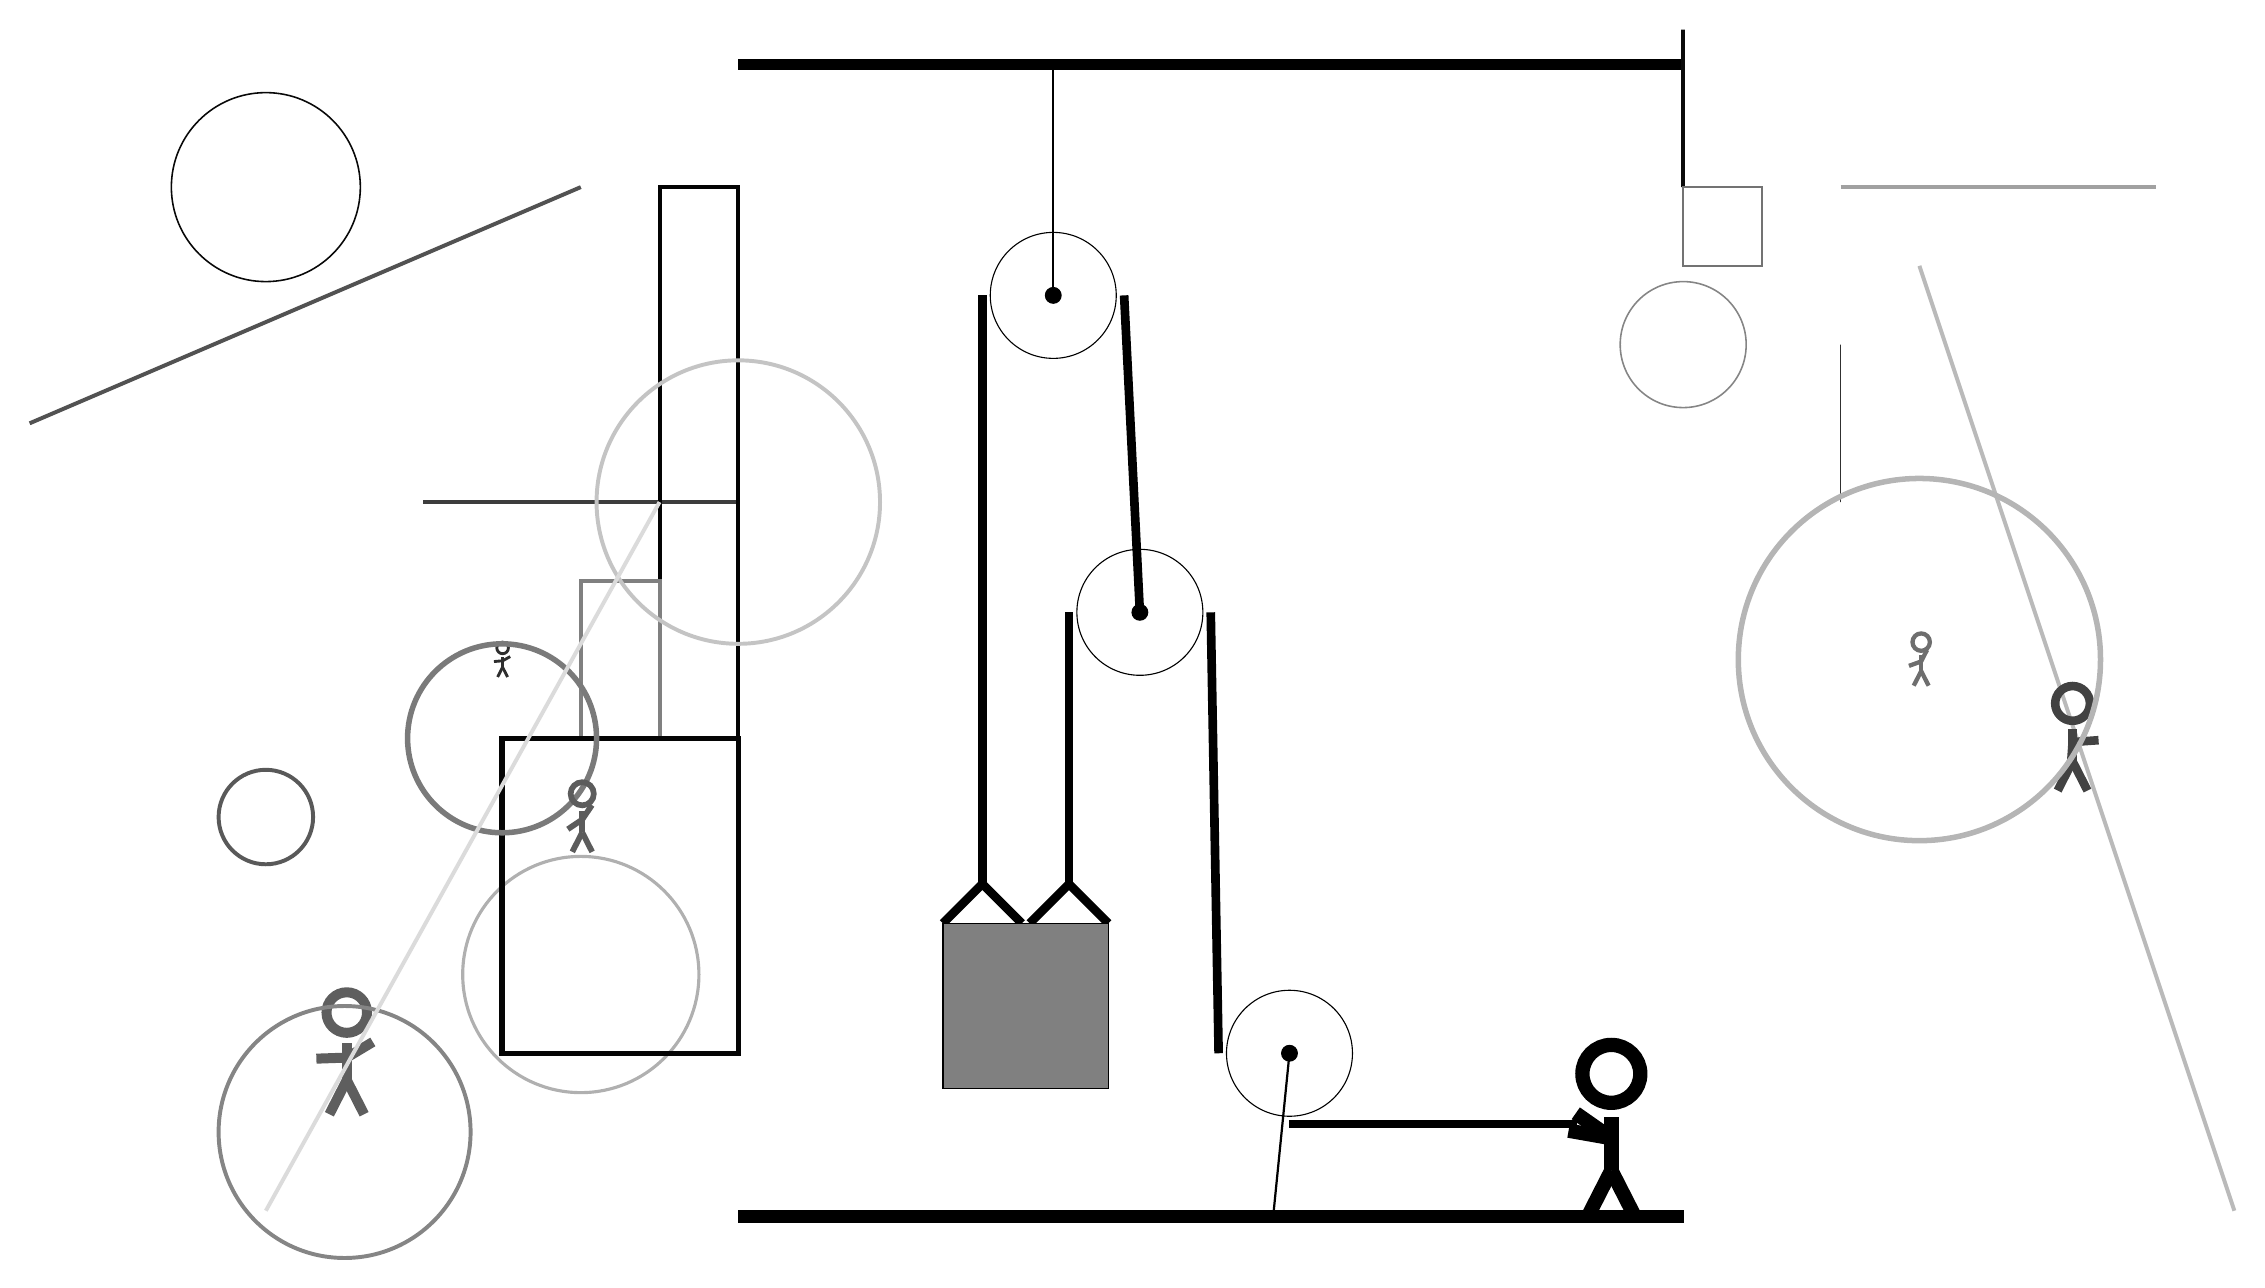
\begin{tikzpicture}
			%%%%% START %%%%%
			
			\draw[fill=black] (-2, 11.5) rectangle (10, 11.625);
			
			\draw (2, 8.625) circle (0.8);
			\draw[fill=black] (2, 8.625) circle (0.1);
			\draw[thick] (2, 8.625) -- (2, 11.5);
			
			\draw (3.1, 4.6) circle (0.8);
			\draw[fill=black] (3.1, 4.6) circle (0.1);
			
			\draw[line width=0.5mm, color=black!76](-6, 6) -- (-2, 6);
			
			\draw[line width=0.5mm, color=black!99] (-3, 3) rectangle (-2, 10);
			\draw[line width=0.2mm, color=black!81] (12, 8) rectangle (12, 6);
			\node[line width=0.6mm, color=black!63] at (-7, -1) {\Strichmaxerl[7][2][31]};
			
			\node[line width=0.5mm, color=black!82] at (-5, 4) {\Strichmaxerl[2][5][29]};
			
			\draw [line width=0.5mm, color=black!48](-7, -2) circle (1.6);
			\draw [line width=0.2mm, color=black!97](-8, 10) circle (1.2);
			
			\draw [line width=0.2mm, color=black!48](10, 8) circle (0.8);
			\draw[line width=0.5mm, color=black!27](13, 9) -- (17, -3);
			\draw[line width=0.5mm, color=black!96] (10, 12) rectangle (10, 10);
			\draw[line width=0.2mm, color=black!55] (11, 9) rectangle (10, 10);
			\node[line width=0.6mm, color=black!74] at (15, 3) {\Strichmaxerl[6][86][4]};
			\node[line width=0.7mm, color=black!57] at (13, 4) {\Strichmaxerl[3][20][63]};
			
			\draw[line width=0.5mm, color=black!50] (-4, 5) rectangle (-3, 3);
			\draw [line width=0.4mm, color=black!31](-4, 0) circle (1.5);
			\draw [line width=0.5mm, color=black!65](-8, 2) circle (0.6);
			
			\draw [line width=0.5mm, color=black!23](-2, 6) circle (1.8);
			\draw[line width=0.7mm, color=black!98] (-2, 3) rectangle (-5, -1);
			\draw[line width=0.5mm, color=black!68](-4, 10) -- (-11, 7);
			\draw [line width=0.7mm, color=black!52](-5, 3) circle (1.2);
			\draw [line width=0.7mm, color=black!29](13, 4) circle (2.3);
			
			\draw[line width=0.5mm, color=black!37](12, 10) -- (16, 10);
			\draw[line width=0.5mm, color=black!14](-3, 6) -- (-8, -3);
			\node[line width=0.3mm, color=black!64] at (-4, 2) {\Strichmaxerl[4][34][56]};
			\draw[line width=0.4mm, color=black!80] (-2, 10) rectangle (-2, 10);
			
			\draw (5, -1) circle (0.8);
			\draw[fill=black] (5, -1) circle (0.1);
			\draw[thick] (5, -1) -- (4.8, -3);
			
			\draw[line width = 1.1mm]  (0.6, 0.65) -- (1.1, 1.15) -- (1.6, 0.65);
			\draw[line width = 1.1mm]  (1.7, 0.65) -- (2.2, 1.15) -- (2.7, 0.65);
			\draw[fill=black!50] (0.6, 0.65) rectangle (2.7, -1.45);
			
			\draw[line width = 1.1mm] (1.1, 8.625) -- (1.1, 1.15);
			\centerarc[line width = 1.1mm](2, 8.625)(0:180:0.9);
			\draw[line width = 1.1mm] (2.9, 8.625) -- (3.1, 4.6);
			\draw[line width = 1.1mm] (2.2, 4.6) -- (2.2, 1.15);
			\centerarc[line width = 1.1mm](3.1, 4.6)(0:180:0.9);
			\draw[line width = 1.1mm] (4.0, 4.6) -- (4.1, -1);
			\centerarc[line width = 1.1mm](5, -1)(180:270:0.9);
			\draw[line width = 1.1mm] (5, -1.9) -- (8.65, -1.9);
			
			\node at (9, -2) {\Strichmaxerl[10][-35][170]};
			
			\draw[fill=black] (-2, -3) rectangle (10, -3.15);
			
			%%%%% END %%%%%
		\end{tikzpicture}
	\end{figure}	
\end{document}